\begin{frame}{Vergleichsgrafiken und Thresholds}
\begin{columns}[T,onlytextwidth]
\begin{column}{0.5\textwidth}
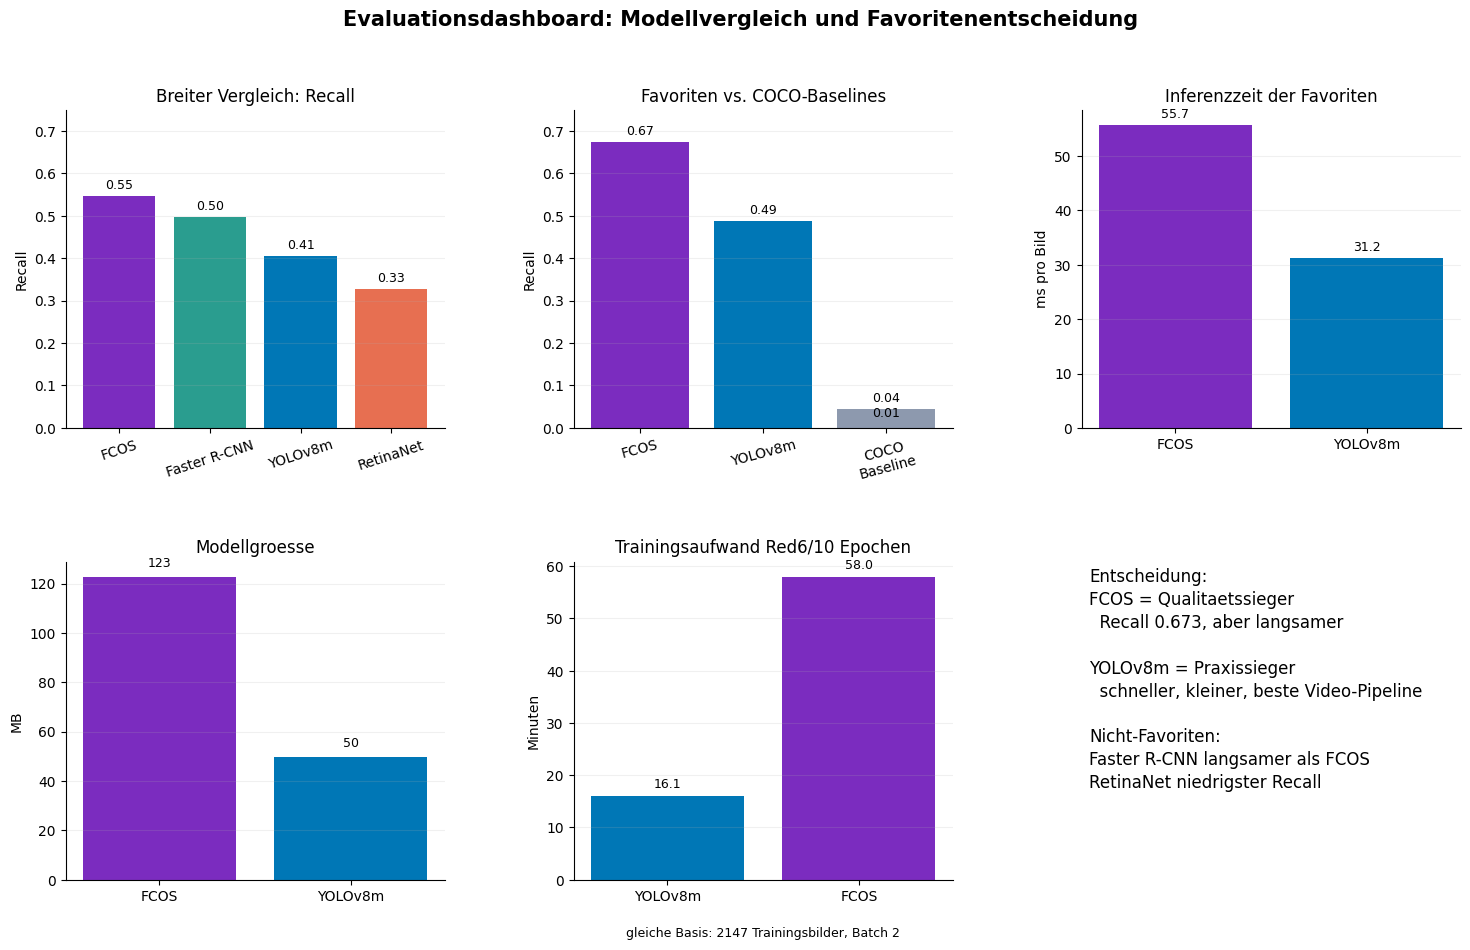
\includegraphics[width=\textwidth,height=0.47\textheight,keepaspectratio]{imglib/face_model_lab/evaluationsdashboard.png}
\end{column}
\begin{column}{0.48\textwidth}
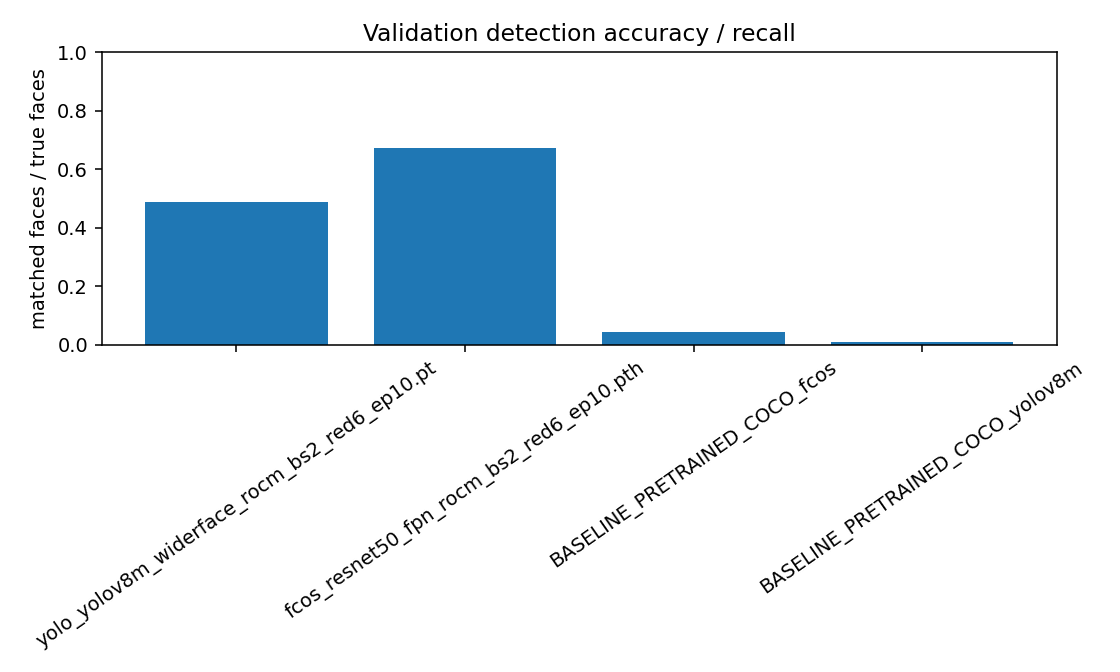
\includegraphics[width=\textwidth,height=0.23\textheight,keepaspectratio]{imglib/face_model_lab/red6_validation_recall.png}
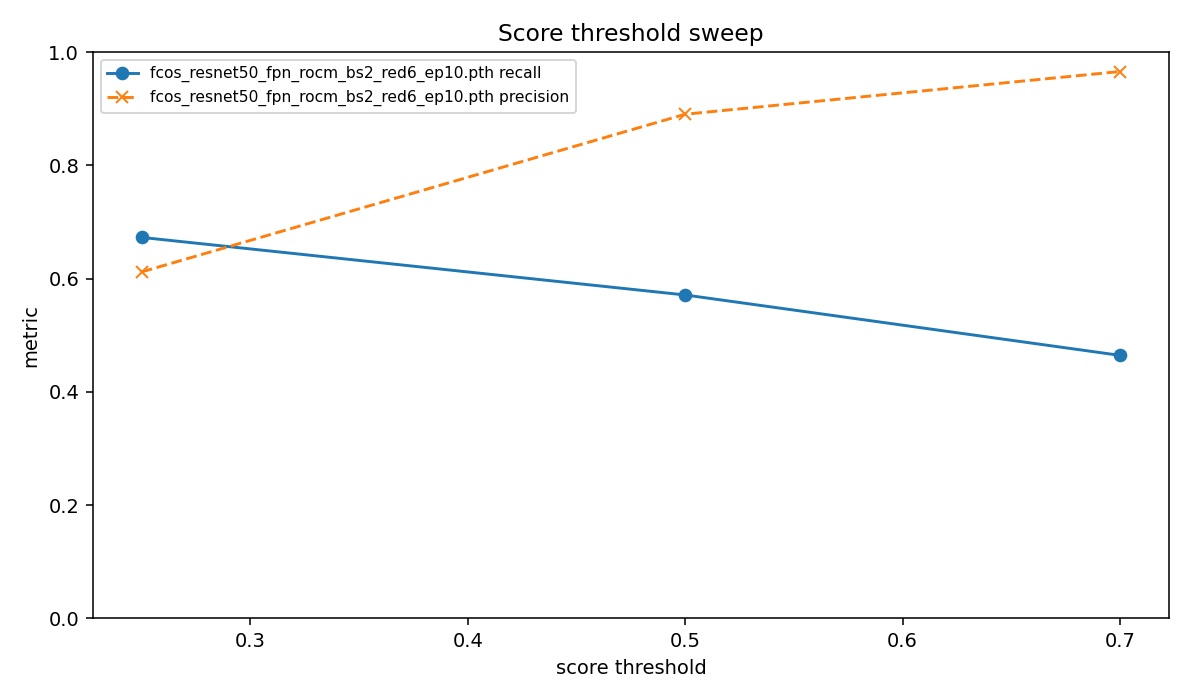
\includegraphics[width=\textwidth,height=0.23\textheight,keepaspectratio]{imglib/face_model_lab/red6_threshold_sweep.png}
\end{column}
\end{columns}
\vspace{0.4em}
\small
\begin{itemize}
    \item Hoehere Thresholds reduzieren Fehlalarme; gleichzeitig sinkt der Recall.
    \item Fuer Datenschutz ist ein niedrigerer Threshold plausibel, weil uebersehene Gesichter kritischer sind.
\end{itemize}
\end{frame}
